\documentclass[tikz,border=6pt]{standalone}
\usepackage{tikz}
\usetikzlibrary{arrows.meta,positioning}

\begin{document}
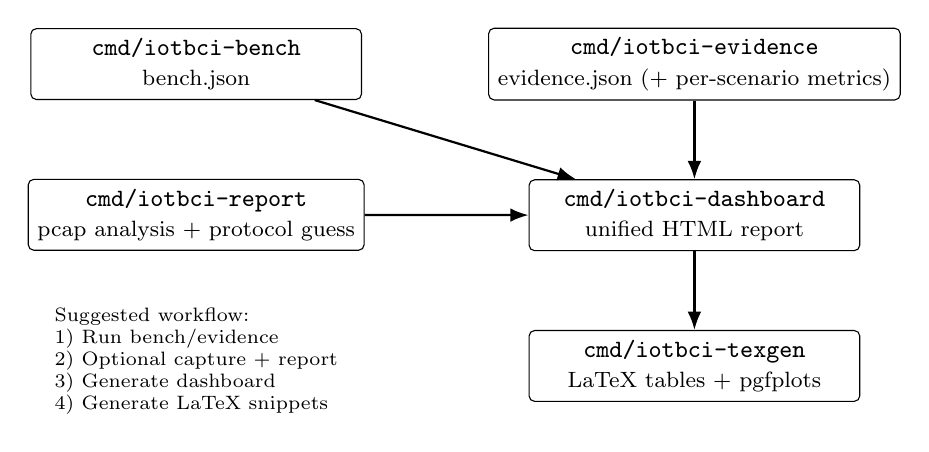
\begin{tikzpicture}[
  font=\small,
  box/.style={draw,rounded corners=2pt,minimum width=4.2cm,minimum height=0.9cm,align=center},
  arrow/.style={-Latex,thick},
]
  \node[box] (bench) {\texttt{cmd/iotbci-bench}\\\footnotesize bench.json};
  \node[box,right=1.6cm of bench] (evidence) {\texttt{cmd/iotbci-evidence}\\\footnotesize evidence.json (+ per-scenario metrics)};
  \node[box,below=1.0cm of bench] (report) {\texttt{cmd/iotbci-report}\\\footnotesize pcap analysis + protocol guess};
  \node[box,below=1.0cm of evidence] (dash) {\texttt{cmd/iotbci-dashboard}\\\footnotesize unified HTML report};
  \node[box,below=1.0cm of dash] (texgen) {\texttt{cmd/iotbci-texgen}\\\footnotesize LaTeX tables + pgfplots};

  \draw[arrow] (bench) -- (dash);
  \draw[arrow] (evidence) -- (dash);
  \draw[arrow] (report) -- (dash);
  \draw[arrow] (dash) -- (texgen);

  \node[font=\scriptsize,align=left,below=0.6cm of report] {
    Suggested workflow:\\
    1) Run bench/evidence\\
    2) Optional capture + report\\
    3) Generate dashboard\\
    4) Generate LaTeX snippets
  };
\end{tikzpicture}
\end{document}

